\documentclass[12pt,twoside]{reedthesis}
\usepackage{graphicx,latexsym} 
\usepackage{amssymb,amsthm,amsmath}
\usepackage{longtable,booktabs,setspace} 
\usepackage[hyphens]{url}
\usepackage{rotating}
\usepackage{natbib}
% Comment out the natbib line above and uncomment the following two lines to use the new 
% biblatex-chicago style, for Chicago A. Also make some changes at the end where the 
% bibliography is included. 
%\usepackage{biblatex-chicago}
%\bibliography{thesis}

\usepackage{graphicx}
% \usepackage{times} % other fonts are available like times, bookman, charter, palatino

\title{My Final College Paper}
\author{Your R. Name}
% The month and year that you submit your FINAL draft TO THE LIBRARY (May or December)
\date{May 200x}
\division{Mathematics and Natural Sciences}
\advisor{Advisor F. Name}
%If you have two advisors for some reason, you can use the following
%\altadvisor{Your Other Advisor}
%%% Remember to use the correct department!
\department{Mathematics}

\setlength{\parskip}{0pt}
%%
%% End Preamble
%%
%% The fun begins:
     
     \newenvironment{halfpage}{
         \begin{minipage}{0.5\textwidth}
     }
     {
         \end{minipage}
     }

\usepackage{braket}
\usepackage{tristan-math}
\theoremstyle{definition}\newtheorem{definition}{Definition}


\usetikzlibrary{arrows, shapes.gates.logic.US, calc}
\begin{document}

% \textbf{Some background:} Quantum Mechanics came into prevalence in the early 1900s. 

\section{Classical Computation and Information}
Before we begin with \emph{quantum} computation, we should first give a quick overview of \emph{classical} computing. There are many different models for classical computing. The most famous perhaps is the turing-machine or the von-Neumman architecture (this is what most actual computers are modeled after).


In practice, most algorithms are studied in programming languages or psuedocode. However, we will focus on the \emph{circuit model} of computation which will give us a more natural framework to generalize into the quantum setting.

Before we get to circuits, we first need to introduce \emph{logic gates} and \emph{bits}:


%% TODO, explain this better
\begin{definition}
    A \emph{bit} is any element $b \in \Z/2\Z$. We will express $b$ as either 0 or 1, although at times it may be convenient to think of a bit as true or false.
\end{definition}

Logic gates correspond to boolean operations.

\vfill
\pagebreak




\textbf{A Motivating Example} \\
Suppose I have two boxes. I write down my two favorite integers on separate pieces of paper and lock them in different boxes. Your goal is to determine whether the sum of the two numbers is even or odd. I will open the boxes for you if you really want me to, but I really don't like opening boxes (perhaps I have a bad childhood memory relating to boxes). How many boxes do you need me to open to answer the problem?

\textbf{The Bit} \\
The fundamental unit of information is the bit. The term bit was introduced by Claude Shannon in 1948. It was a contraction of ``binary information digit''. A bit is the smallest nontrivial unit of information.

A bit $b$ has two possible states. Generally, this is represented as
\[
    b \in \{0, 1\} \cong \{\text{True},\ \text{False}\} \simeq \Z/2\Z
\]
Sometimes thinking of a bit as true/false is helpful.

Importantly, we can have a list of several bits. A string $s$ (of length $n$) is an ordered tuple of $n$-bits. This is expressed as a cartesian product
\[
    s \in \{0, 1\}^n \cong (\Z/2\Z)^n
\]


\textbf{Logic Gates and Bit Operations} \\
We can perform operations on bits. We will express these as logic gates. If you've done propositional logic in a philosophy or math class, this is the same system just with different notation.

We start with the unary gates. These take one bit as input and return one bit. Here is a $\texttt{NOT}$ gate:
\begin{center}
    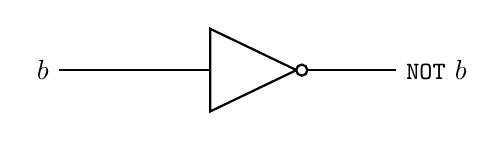
\begin{tikzpicture}[thick]
        \node (b) at (0, 0) {$b$};
        \node (bout) at (5,0) {\texttt{\small NOT} $b$};
        \node[not gate US, draw, minimum size=0.9cm] at ($(b) + (2.5, 0)$) (notb) {};
        \draw (b) -- (notb.input);
        \draw (notb.output) -- (bout);
    \end{tikzpicture}
    
\end{center}

It takes 0 to 1 and 1 to 0. It can be defined by the truth table:
\begin{tabular}{l|l}
0 & 1 \\
1 & 0
\end{tabular}

There are in fact 4 unary gates, one for each of the 4 truth tables. Writing them out is a good exercise. Importantly More generally, the logic of any circuit is nothing more or less than a truth table. Here is an arbitrary circuit:
\begin{center}
    \hspace{12mm}
    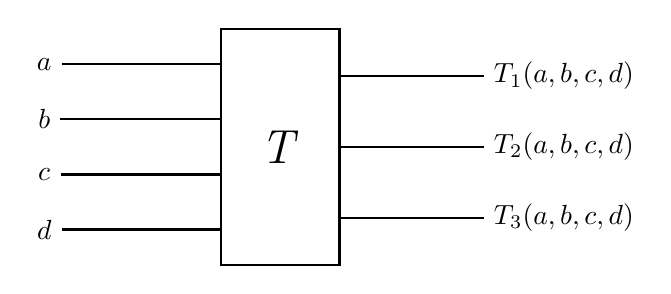
\begin{tikzpicture}[thick]
        \node (a) at (1, 3.05) {$a$};
        \node (b) at (1, 2.35) {$b$};
        \node (c) at (1, 1.65) {$c$};
        \node (d) at (1, 0.95) {$d$};

        \node (x) at (7.6, 2.9) {$T_1(a, b, c, d)$};
        \node (y) at (7.6, 2) {$T_2(a, b, c, d)$};
        \node (z) at (7.6, 1.1) {$T_3(a, b, c, d)$};

        \node (rect) at (4,2) [draw,thick,minimum width=1.5cm,minimum height=3cm] {\textit{\LARGE T}};

        \draw (a) -- (3.24, 3.05);
        \draw (b) -- (3.24, 2.35);
        \draw (c) -- (3.24, 1.65);
        \draw (d) -- (3.24, 0.95);
        \draw (4.76, 2.9) -- (x);
        \draw (4.76, 2) -- (y);
        \draw (4.76, 1.1) -- (z);
    \end{tikzpicture}
\end{center}
In this case $T : \{0,1\}^4 \rightarrow \{0,1\}^3$ takes as input 4 bits and returns 3 bits. I use the variable $T$ to emphasize that could be thought of as a truth table.



There are two-bit gates $\texttt{AND}$ and $\texttt{XOR}$. The fancy symbol here $\oplus$ means $\texttt{XOR}$. It gets a special symbol because it has the special property of being linear. In fact, it is just addition mod 2. \\

\begin{halfpage}
    \centering
    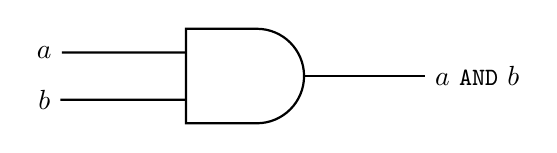
\begin{tikzpicture}[thick]
        \node (x) at (0, 0.8) {$a$};
        \node (y) at (0, 0.2) {$b$};
        \node (output) at (5.5,0.5) {$a$ \texttt{\small AND} $b$};

        \node[and gate US, draw, rotate=0, logic gate inputs=222, minimum size=1.2cm] at ($(2.5, 0.5)$) (xory) {};
        \draw (x) -- (xory.input 1);
        \draw (y) -- (xory.input 3);

        \draw (xory.output) -- (output);
    \end{tikzpicture}
\end{halfpage}
\begin{halfpage}
    \centering
    \begin{tikzpicture}[thick]
        \node (x) at (0, 0.8) {$a$};
        \node (y) at (0, 0.2) {$b$};
        \node (output) at (5.5,0.5) {$a$ \oplus \  $b$};


        \node[xor gate US, draw, rotate=0, logic gate inputs=22, minimum size=1.2cm] at ($(2.5, 0.5)$) (xory) {};
        \draw (x) -- (1.74, 0.8);
        \draw (y) -- (1.74, 0.2);

        \draw (xory.output) -- (output);
    \end{tikzpicture}
\end{halfpage}

I should mention that you can build any arbitrary circuit using \texttt{AND} and \texttt{NOT}.\,  Here are two examples, \texttt{Controlled AND} and \texttt{Controlled XOR} \\


    \begin{halfpage}
    

    \begin{center}
      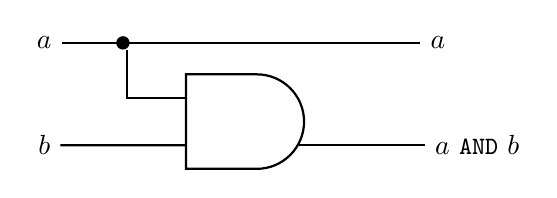
\begin{tikzpicture}[thick]
        \node (x) at (0, 1.5) {$a$};
        \node (y) at (0, 0.2) {$b$};
        \node[circle, fill=black, inner sep=0pt, minimum size=1.7mm] (c) at (1, 1.5) {};
        \node (output) at (5.5,0.2) {$a$ \texttt{\small AND} $b$};
        \node (aout) at (5,1.5){$a$};
 
        \node[and gate US, draw, rotate=0, logic gate inputs=222, minimum size=1.2cm] at ($(2.5, 0.5)$) (xory) {};
        \draw (x) -- (c);
        \draw (c) -- ([xshift=0.4cm]c) |- (xory.input 1);
        \draw (y) -- (xory.input 3);
        \draw (x) -- (aout);
        \draw (3.23,0.2) -- (output);
    \end{tikzpicture}
    \end{center}
    \end{halfpage}
    \begin{halfpage}
    \begin{center}
            \begin{tikzpicture}[thick]
        \node (x) at (0, 1.5) {$a$};
        \node (y) at (0, 0.2) {$b$};
        \node (aout) at (5,1.5){$a$};
        \node (output) at (5.5,0.5) {$a$ \oplus \  $b$};
        \node[circle, fill=black, inner sep=0pt, minimum size=1.7mm] (c) at (1, 1.5) {};

        \node[xor gate US, draw, rotate=0, logic gate inputs=22, minimum size=1.2cm] at ($(2.5, 0.5)$) (xory) {};
        \draw (x) -- (c);
        \draw (c) -- (aout);
        \draw (y) -- (1.74, 0.2);
        \draw (c) -- ([xshift=0.4cm]c) |- (1.74, 0.8);
        \draw (xory.output) -- (output);
    \end{tikzpicture}
    \end{center}
    \end{halfpage}

    The second one, \texttt{Controlled XOR} is $\textit{reversible}$. If we apply it twice, we get the identity. Such gates are classically important because they don't add entropy and thus generate less heat.


    \begin{center}
        \textbf{\Large Quantum Computing and Quantum Information} \\
    \end{center}
        \bigskip 

    \textbf{The Qubit} \\
    \textit{Background: Just as the bit is the fundamental unit of information, the qubit is the fundamental unit of quantum information. It represents the state of a 2 state quantum mechanical system (the simplest nontrivial quantum system)}

    A classical bit is either 0 or 1. A qubit is a pair of complex numbers 
    \[
        (\alpha, \beta) \in \C^2 
    \]
    satisfying the condition
    \[
        |\alpha|^2 + |\beta|^2 = 1
    \]
    Importantly, $\C^2$ is a 2-dimensional complex vector space and it has an orthonormal basis   \[
        \left\{\cvec{0}{1}, \cvec{1}{0}\right\}
    \]
    In physics notation, we call these vectors $\ket{0}$ and $\ket{1}$, respectively.\\ 

    \textit{Examples:}

    \textbf{Multiple Qubits}\\ 
    We can also have multiple qubit strings. They are expressed as a tensor product. A two qubit string is a vector in $\C^2 \otimes \C^2$ and an $n$ cubit string is a vector in $(\C^2)^{\otimes n}$. This may seem odd, especially if you are not familiar with the tensor product. However, there is good motivation for it. An important property of the tensor product, is that for two vector spaces $V$, $W$
    \[
        \dim (V \otimes W ) = \dim(V)\dim(W)
    \]
    Therefore just as an $n$-bit string has $2^n$ possible states, an $n$-qubit string lives in a $2^n$ dimensional complex vector space. Although we can draw a (limited) picture for one qubit, it quickly becomes impossible even for two qubits.

    You may ask why a qubit lives in $\C^2$. That is a good question that I would recommend asking a physicist. 
    This does raise an issue though. $\C^2$ is a continuous vector space. This means that we couldn't even write down the state of a qubit as a finite number of classical bits. 


    \textbf{Quantum Gates and Qubit Operations} \\
    There is one special qubit operation that is different from the rest, called measurement. It resolves this infinite information paradox we have run into.

    When we measure a qubit, it ``collapses'' into a classical bit. It becomes $\ket{0}$ with probability $|\alpha|^2$ and $\ket{1}$ with probability $|\beta|^2$. In math notation this is

    \[
        \textsf{Measure}\left[\alpha\cvec{0}{1} + \beta\cvec{1}{0}\right] = 
        \begin{cases}
            \cvec{0}{1} &\text{with probability } |\alpha|^2 \vspace{5px}\\
            \cvec{1}{0} &\text{with probability } |\beta|^2
        \end{cases}
    \]
\end{document}